\documentclass[conference]{IEEEtran}
\IEEEoverridecommandlockouts
% The preceding line is only needed to identify funding in the first footnote. If that is unneeded, please comment it out.
\usepackage{cite}
\usepackage{amsmath,amssymb,amsfonts}
\usepackage{algorithmic}
\usepackage{graphicx}
\usepackage{textcomp}
\usepackage{xcolor}
\def\BibTeX{{\rm B\kern-.05em{\sc i\kern-.025em b}\kern-.08em
		T\kern-.1667em\lower.7ex\hbox{E}\kern-.125emX}}
\begin{document}
	
\title{Enhancing Reasoning Skills in Small Persian Medical Language Models Can Outperform Large-Scale Data Training}
	
\author{\IEEEauthorblockN{1\textsuperscript{st} Mehrdad Ghassabi}
		\IEEEauthorblockA{\textit{Faculty of Computer Engineering} \\
			\textit{University of Isfahan}\\
			Isfahan, Iran \\
			m.ghassabi@eng.ui.ac.ir}
		\and
		\IEEEauthorblockN{2\textsuperscript{nd} Sadra Hakim}
		\IEEEauthorblockA{\textit{School of Computer Science} \\
			\textit{University of Windsor}\\
			Windsor, Canada \\
			hakim6@uwindsor.ca}
		\and
		\IEEEauthorblockN{3\textsuperscript{rd} Hamidreza Baradaran Kashani}
		\IEEEauthorblockA{\textit{Faculty of Computer Engineering} \\
			\textit{University of Isfahan}\\
			Isfahan, Iran \\
			hrb.kashani@eng.ui.ac.ir }
		\and
		\IEEEauthorblockN{4\textsuperscript{th} Pedram Rostami}
		\IEEEauthorblockA{\textit{School of Electrical and Computer Engineering} \\
			\textit{University of Tehran}\\
			Tehran, Iran \\
			pedram.rostami@ut.ac.ir}
	}
	
	\maketitle
	
	\begin{abstract}
Enhancing reasoning capabilities in small language models is critical for specialized applications such as medical question answering, particularly in underrepresented languages like Persian. In this study, we employ Reinforcement Learning with AI Feedback (RLAIF) and Direct preference optimization (DPO) to improve the reasoning skills of a general-purpose Persian language model. To achieve this, we translated a multiple-choice medical question-answering dataset into Persian and used RLAIF to generate rejected-preferred answer pairs, which are essential for DPO training. By prompting both teacher and student models to produce Chain-of-Thought (CoT) reasoning responses, we compiled a dataset containing correct and incorrect reasoning trajectories. This dataset, comprising 2 million tokens in preferred answers and 2.5 million tokens in rejected ones, was used to train a baseline model, significantly enhancing its medical reasoning capabilities in Persian. Remarkably, the resulting model outperformed its predecessor, gaokerena-V, which was trained on approximately 57 million tokens, despite leveraging a much smaller dataset. These results highlight the efficiency and effectiveness of reasoning-focused training approaches in developing domain-specific language models with limited data availability.
	\end{abstract}
	
	\begin{IEEEkeywords}
		system2 deep learning,small language model,medical language models, RLAIF, direct policy optimization
	\end{IEEEkeywords}
	
	\section{Introduction}
In 2019, at the NeurIPS conference, Yoshua Bengio highlighted a critical limitation of current deep learning systems: their inability to perform tasks requiring robust reasoning skills
\cite{b1}.
While these systems excel at intuitive, perception-driven tasks, they struggle with reasoning-based challenges that demand deeper cognitive processing. This observation echoes Daniel Kahneman’s distinction between “fast” and “slow” thinking in cognitive science
\cite{b2}.
Fast, intuitive thinking aligns with the strengths of current AI systems, whereas slow, deliberate reasoning remains a significant weakness.

One proposed solution to this deficiency is the revival of symbolic AI methods through neurosymbolic approaches. However, Bengio cautioned against such methods due to scalability issues. Instead, he urged the development of new architectures capable of out-of-distribution generalization—a core requirement for genuine reasoning.

The Transformer architecture
\cite{b3}, which underpins most modern language models, suffers from the same deficiency. Transformers often make “stupid mistakes” when faced with reasoning-intensive problems, prompting researchers to enlarge models and datasets in an attempt to achieve better results across tasks. This approach arguably simulates System 2 reasoning within a fundamentally System 1 framework.

This limitation becomes even more pronounced in smaller language models, where restricted capacity and limited data exacerbate reasoning challenges. In domains such as medicine—where reasoning, interpretation, and decision-making are essential—these weaknesses become especially consequential.

Recent efforts to enhance reasoning have largely focused on prompting or fine-tuning methods that enable models to imitate reasoning behavior rather than truly engage in it—a phenomenon we refer to as the “illusion of thinking”
\cite{b4}.
In the absence of architectures with intrinsic reasoning capabilities, such approaches provide only an approximation of genuine cognitive reasoning. Nevertheless, these efforts represent necessary steps toward achieving more reasoning-capable AI systems.

The present work aims to address this challenge by enhancing the reasoning abilities of a small Persian language model, aya-expanse-8b
\cite{b5}. We first prompt the model to generate Chain-of-Thought (CoT) trajectories for multiple-choice medical questions. These responses are then reviewed and corrected using DeepSeek-R, a model adept at reasoning, to rectify errors. This process constitutes Reinforcement Learning with AI Feedback (RLAIF)
\cite{b6}. By pairing incorrect and corrected CoT trajectories, we subsequently apply Direct Preference Optimization (DPO)
\cite{b7} to enhance the reasoning capabilities of the baseline model.

We call this improved model gaokerena-R. While its predecessor, gaokerena-V
\cite{b8}, demonstrated superior medical knowledge in straightforward prompting tasks, gaokerena-R outperformed it when evaluated using Chain-of-Thought (CoT) prompting
\cite{b9}. Notably, gaokerena-R was trained on a much smaller dataset, focusing on reasoning enhancement rather than data scale, whereas gaokerena-V relied on extensive training on a large medical corpus and the MF3QA dataset
\cite{b8}.

Our findings highlight an important insight: in low-resource domains such as Persian medical AI, strengthening reasoning capabilities can be more effective than training on vast datasets. This underscores the importance of developing reasoning-oriented approaches, particularly in languages and fields with limited data availability. By improving reasoning abilities in smaller models, we can make meaningful progress toward practical, resource-efficient AI systems.
	
	\section{Related Work}
To the best of our knowledge, no prior work has focused on developing Persian medical reasoning language models. Existing Persian medical models, including our previous gaokerena-V, mainly address knowledge representation and general language understanding with limited attention to reasoning.

 L. Pan et al. reviewed several valuable studies on enhancing reasoning capabilities in language models.
\cite{b10}
Accordingly, we focus here on English-language works that offer methodological insights into generating and integrating reasoning data for improving medical language models.
	\subsection{Related Work In Medical Domain}
One of the notable efforts in developing small-scale medical reasoning language models is MedSSS
\cite{b11}.
This framework focuses on fine-graining the intermediate reasoning steps to enhance the reasoning ability of medical models. To accomplish this, the authors applied the Monte Carlo Tree Search (MCTS)
\cite{b12}
algorithm on medical multiple-choice question-answering datasets to synthesize structured reasoning trajectories using a policy model. Based on this approach, they constructed three datasets supporting different stages of training: a dataset for Supervised Fine-Tuning (SFT) of the policy model, a rejected–preferred answer dataset for Direct Preference Optimization (DPO)
\cite{b13}
,and a soft dual-side label dataset for fine-tuning the Process Reward Model (PRM).Finally, the trained Policy Model was used as the primary reasoning policy, while the trained Process Reward Model acted as a decoding guide to refine and evaluate the reasoning process during generation.

Another significant contribution in this field is MedReason
\cite{b14}. 
In this work, the authors leveraged a structured medical knowledge graph to transform conventional question–answer (Q\&A) pairs into detailed medical reasoning trajectories. Each trajectory represented the step-by-step logical pathway connecting a clinical question to its correct answer, grounded in medical knowledge relationships such as symptoms, diagnoses, treatments, and physiological mechanisms. By constructing a reasoning-enriched dataset in this manner, the authors were able to fine-tune a baseline language model on these structured reasoning examples. This approach led to a marked improvement in the model’s ability to perform reasoning-intensive tasks within the medical domain, demonstrating the effectiveness of incorporating knowledge graph–based reasoning supervision into the training process. The findings from MedReason further emphasize the importance of structured reasoning representations as a means of improving the interpretability and analytical depth of medical language models.

Another important advancement in the development of medical reasoning models is HuatuoGPT-o1
\cite{b15}. 
In this work, the authors introduced a verification-guided reasoning framework designed to improve the logical consistency and accuracy of generated reasoning trajectories. Specifically, they employed a verifier model to assess and guide the policy model during reasoning generation, ensuring that each reasoning path adhered closely to factual correctness and medical plausibility. By filtering and refining reasoning trajectories through this verification process, they created a high-quality dataset composed of verified reasoning sequences. The authors then leveraged both supervised fine-tuning and reinforcement learning techniques to train their baseline language model using these verified data. This dual training approach allowed the model to not only imitate correct reasoning behaviors but also internalize reasoning principles through reward-driven optimization. As a result, HuatuoGPT-o1 demonstrated significant improvements in reasoning accuracy and reliability across a variety of medical question-answering and diagnostic tasks, highlighting the potential of verifier-guided learning frameworks in advancing medical reasoning language models.


         \subsection{Related Work In Other Domain}
Perhaps the most influential recent work in the broader field of AI reasoning is DeepSeek-R
\cite{b16}. Building upon the DeepSeek-V3-Base model, the authors introduced a reinforcement learning framework based on Gradient Regularized Policy Optimization (GRPO)
\cite{b17} 
to explicitly enhance the model’s reasoning capabilities. In this setup, the reinforcement learning process was guided by a reward function specifically designed to evaluate and maximize reasoning performance. Through this training paradigm, DeepSeek-R demonstrated remarkable improvements in logical reasoning and problem-solving accuracy across various benchmarks.  
However, the application of reinforcement learning also introduced several side effects. While reasoning performance improved substantially, the model’s readability and linguistic coherence deteriorated, and instances of language mixing became more frequent. To address these issues, the authors incorporated a small amount of cold-start supervised data and adopted a multi-stage training pipeline. This additional fine-tuning phase helped restore natural language fluency and readability while retaining the strong reasoning skills acquired through reinforcement learning. The resulting model, DeepSeek-R, thus represents a critical step forward in reasoning-oriented AI, demonstrating that reinforcement learning can significantly enhance reasoning ability—provided it is balanced with targeted fine-tuning to maintain linguistic quality.

Another notable contribution in the area of reasoning enhancement is Thought Preference Optimization (TPO)
\cite{b18}. 
In this work, the authors proposed a preference-based framework for improving reasoning quality in language models. Given a question, the model first generates multiple candidate reasoning trajectories. These responses are then evaluated by a judge model, which identifies the best and worst samples based on reasoning correctness and coherence. The collected best–worst pairs are subsequently used to train the baseline model through Direct Preference Optimization (DPO), encouraging it to prefer higher-quality reasoning paths. This approach effectively aligns the model’s reasoning process with human-like evaluative feedback, demonstrating that reasoning quality can be substantially improved through structured preference optimization rather than relying solely on scale or supervised data.

Another relevant study was conducted by N. Ho et al.
\cite{b19},
who explored the transfer of reasoning capabilities from large language models to smaller ones. In their approach, a smaller model was fine-tuned using data generated by a larger model that exhibited stronger reasoning performance. The larger model produced reasoning trajectories and question–answer pairs that served as high-quality supervision signals for the smaller model. Through this distillation process, the smaller model effectively learned reasoning strategies and problem-solving patterns from its larger counterpart, achieving competitive reasoning performance with significantly reduced computational cost. This work demonstrates that reasoning ability can be efficiently transferred across models of different scales through targeted fine-tuning on reasoning-oriented synthetic data.
          \section{Proposed Methods}
We proposed two methods. The first framework, depicted in \ref{fig1}, utilizes a teacher model ( we used DeepSeek-R), which is itself a reasoning language model, to correct the student model’s medical reasoning mistakes. When provided with the correct answer, the teacher generates a detailed chain-of-thought explanation that highlights the reasoning behind the solution. In this setup, the teacher’s output serves as the preferred answer, while the student’s original response is treated as the rejected answer for Direct Policy Optimization (DPO).

 The second framework, depicted in \ref{fig2}, employs the teacher model to provide more granular feedback by identifying specific errors in the student model’s answer. Through this constructive criticism, the student model is guided toward producing the correct answer independently. In this case, the final answer generated by the student is considered the preferred response, while its initial attempt functions as the rejected one for DPO. Although the second framework is considerably more time-consuming due to the iterative feedback process, it can significantly enhance the student model’s learning because DPO leverages preferred-rejected answer pairs generated solely by the student itself. Due to hardware limitations, we generated 95\% of the training data using Framework 1 and the remaining 5\% using Framework 2, balancing efficiency with the benefits of student-driven optimization.
\begin{figure}[h]
    \centering
    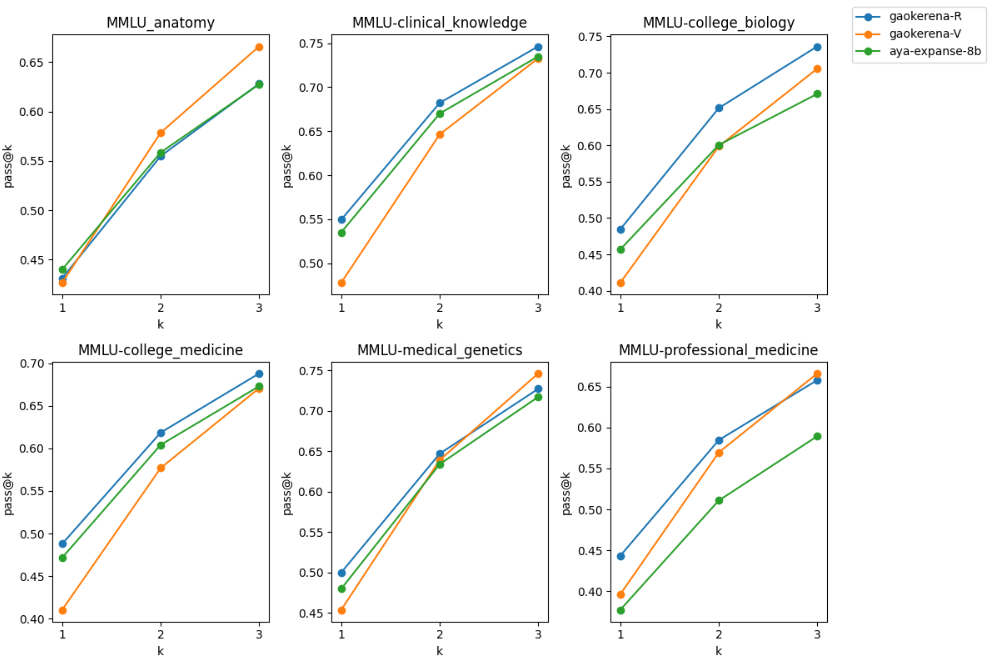
\includegraphics[width=1.0\linewidth]{fig1.png}
    \caption{Framework 1 Block Diagram}
    \label{fig1}
\end{figure}

\begin{figure}[h]
    \centering
    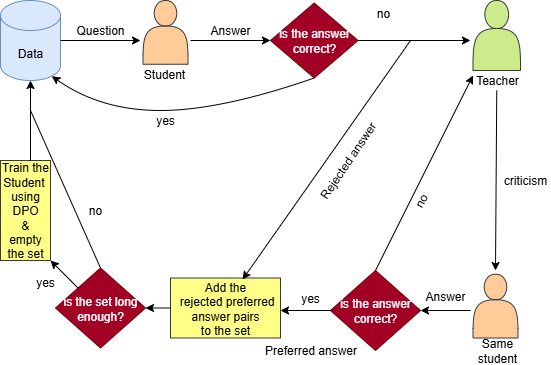
\includegraphics[width=1.0\linewidth]{fig2.png}
    \caption{Framework 2 Block Diagram}
    \label{fig2}
\end{figure}


          \section{Results}
In this section, we compare the newly developed gaokerena-R model with its predecessor, gaokerena-V. While gaokerena-V was trained on a large medical corpus and demonstrates strong factual knowledge and retrieval capabilities, gaokerena-R was specifically designed to enhance medical reasoning. Owing to its reasoning-focused training pipeline, gaokerena-R was trained on a substantially smaller dataset, resulting in slightly reduced coverage of general medical knowledge. However, this trade-off enabled it to develop deeper reasoning competence, allowing it to perform better on tasks requiring multi-step inference and logical consistency.  

In the final evaluation, we compared the performance of gaokerena-V under direct (straight) prompting with that of gaokerena-R when provided with Chain-of-Thought (CoT) prompts. The results highlight that gaokerena-R, despite its smaller scale and limited training data, achieves superior reasoning performance through structured reasoning guidance, demonstrating the effectiveness of reasoning-centered optimization over pure data scaling.
          \subsection{Medical Reasoning Capabillities}
To assess the medical reasoning capabilities of the models, we performed evaluations using the FA\_MED\_MMLU dataset
\footnote{Available at huggingface.co/datasets/gaokerena/FA\_MED\_MMLU}.
 Both gaokerena-V and gaokerena-R were prompted
\footnote{Evaluation prompts are available at github.com/Mehrdadghassabi/Gaokerena-R/blob/main/evaluations/zeroshot-COT/kopp/gaokerena-r1.0/Untitled2.ipynb} 
to generate Chain-of-Thought (CoT) reasoning traces with a temperature setting of 1.0. For each question, five independent samples were generated, and a majority-voting mechanism was applied to determine the final answer: if three or more of the five generations selected the same option, that option was chosen as the final prediction; otherwise, the question was left unanswered to reflect model uncertainty.  

This evaluation framework provides a more robust estimation of reasoning consistency and agreement across multiple reasoning trajectories. The results are presented in Table
\ref{tab:med_reasoning_capabillities_WNM_comparison}
 for the without negative marking setting, and in Table
\ref{tab:med_reasoning_capabillities_NM_comparison}
 for the with negative marking setting. These two scoring schemes allow for a fair comparison of the models’ reasoning accuracy under different evaluation criteria.


	\begin{table}[ht]
		\centering
		\caption{Chain-of-Thought Prompted Performance Without Negative Marking}
		\begin{tabular}{|l|c|c|c|}  
			\hline
			\textbf{} & \textbf{gao} & \textbf{gao} & \textbf{aya-} \\ 
			& \textbf{kerena-R} &  \textbf{kerena-V} & \textbf{expanse-8b} \\
			&   & &(baseline)  \\ \hline
			MMLU- &  &  &  \\ 
			anatomy(fa)  & \textbf{42.22} & 39.25  & 40.74 \\ \hline
			MMLU- &    &  &  \\
			medical-genetics(fa) & \textbf{50.0}  & 41.0  & 45.0 \\ \hline
			MMLU- &  &    &  \\
			college-medicine(fa) & 47.97  & 37.57  &\textbf{48.55}  \\ \hline
			MMLU- &    &  &  \\
			clinical-knowledge(fa)& \textbf{55.84} & 46.79  & 54.71  \\ \hline
			MMLU- &  &  &  \\
			professional-& \textbf{44.85} & 37.13 & 43.75 \\
                        medicine(fa)& &  &  \\ \hline
			MMLU- &  &  &  \\
			college-biology(fa)& \textbf{48.61} & 36.80 & 43.75 \\ \hline
			MMLU(avg) & \textbf{48.76} & 40.40 & 47.10 \\ \hline
			IBMSEE Sept2023 & \textbf{38.69}  & 29.76 & 35.71  \\ \hline
			Number of&  &  &  \\
			parameters & 8b & 8b & 8b \\ \hline
			inference time & $\approx 5 \times 35s$ & $\approx 5 \times 35s$ & $\approx 5 \times 35s$ \\  \hline
		\end{tabular}
		\label{tab:med_reasoning_capabillities_WNM_comparison}
	\end{table}

	\begin{table}[ht]
		\centering
		\caption{Chain-of-Thought Prompted Performance With Negative Marking}
		\begin{tabular}{|l|c|c|c|}  
			\hline
			\textbf{} & \textbf{gao} & \textbf{gao} & \textbf{aya-} \\ 
			& \textbf{kerena-R} &  \textbf{kerena-V} & \textbf{expanse-8b} \\
			&   & &(baseline)  \\ \hline
			MMLU- &  &  &  \\ 
			anatomy(fa)  & \textbf{29.13} & 27.65  & 24.93  \\ \hline
			MMLU- &    &  &  \\
			medical-genetics(fa) & \textbf{40.0}  & 32.0  & 33.0  \\ \hline
			MMLU- &  &    &  \\
			college-medicine(fa) & \textbf{34.68}  & 25.24  & 34.48  \\ \hline
			MMLU- &    &  &  \\
			clinical-knowledge(fa)& \textbf{44.65} & 35.59  & 42.51  \\ \hline
			MMLU- &  &  &  \\
			professional-& \textbf{30.39} & 25.0 & \textbf{30.39}   \\
                        medicine(fa)& &  &  \\ \hline
			MMLU- &  &  &  \\
			college-biology(fa)& \textbf{36.80} & 25.0  & 30.09  \\ \hline
			MMLU(avg) & \textbf{36.14} & 28.57  & 33.55  \\ \hline
			IBMSEE Sept2023 & \textbf{24.60}  & 15.87 & 19.84   \\ \hline
			Number of&  &  &  \\
			parameters & 8b & 8b & 8b \\ \hline
			inference time & $\approx 5 \times 35s$ & $\approx 5 \times 35s$ & $\approx 5 \times 35s$ \\  \hline
		\end{tabular}
		\label{tab:med_reasoning_capabillities_NM_comparison}
	\end{table}
           
           \subsubsection{Pass@K}
The pass@k metric, originally introduced by B. Brown et al.
\cite{b20}, 
provides a robust measure for evaluating language models that generate varying outputs for the same input across multiple samples. It quantifies the probability that a model produces at least one correct answer within \(k\) independent attempts, thereby offering a more comprehensive assessment of reasoning reliability and sample diversity. The formal definition of the metric is as follows, where \(N\) denotes the total number of generated samples and \(C_i\) represents the number of correct samples for problem \(i\):

\begin{equation}
\text{pass@k} = \frac{1}{\text{\# of problems}} \sum_{i=1}^{\text{\# of problems}} \left( 1 -  \frac{\binom{N - C_i}{k}}{\binom{N}{k}} \right)
\end{equation}

Following the same experimental setup described earlier, we computed pass@k scores for \(k = 1, 2, 3\) using both the FA\_MED\_MMLU dataset and the IBMSEE (September 2023) dataset. The evaluation included the gaokerena-R, gaokerena-V, and aya-expanse-8b models. The results for the FA\_MED\_MMLU dataset are illustrated in Figure
\ref{fig3}, while the IBMSEE (September 2023) results are shown in Figure
\ref{fig4}.

As illustrated in Figures
\ref{fig3} and
\ref{fig4}, the gaokerena-R model consistently demonstrated superior performance across nearly all \(k\) values and evaluation categories. This improvement indicates that gaokerena-R possesses more stable and coherent reasoning capabilities, producing correct answers more reliably even with a limited number of samples. In contrast, gaokerena-V exhibited relatively weak performance for smaller \(k\) values, while its results improved as \(k\) increased. This pattern suggests that gaokerena-V is considerably more uncertain when prompted to generate Chain-of-Thought reasoning trajectories, often producing diverse or inconsistent answers across different samples. The results therefore highlight the enhanced reasoning consistency and reliability achieved through gaokerena-R’s targeted reasoning-oriented training approach.


\begin{figure}[h]
    \centering
    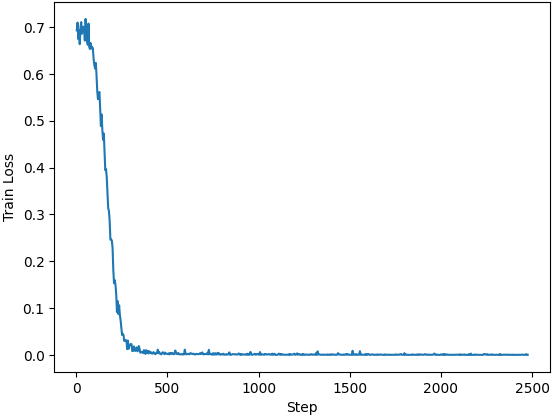
\includegraphics[width=1.0\linewidth]{fig3.png}
    \caption{pass@k results on the FA\_MED\_MMLU dataset using Chain-of-Thought prompting}
    \label{fig3}
\end{figure}

\begin{figure}[h]
    \centering
    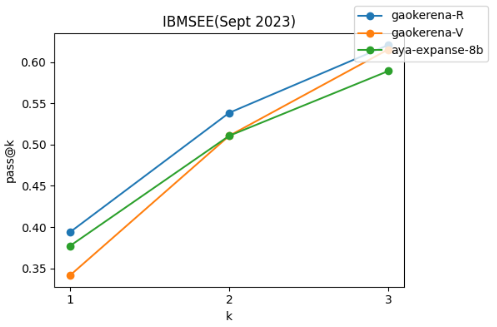
\includegraphics[width=0.8\linewidth]{fig4.png}
    \caption{pass@k results on the IBMSEE (September 2023) dataset using Chain-of-Thought prompting}
    \label{fig4}
\end{figure}

           \subsection{Medical Knowledge}
As mentioned earlier, gaokerena-V possesses a broader base of medical knowledge compared to the newer gaokerena-R model, primarily because it was trained on a significantly larger and more diverse corpus of medical data. This difference becomes evident when both models are evaluated using direct question–answer prompting, rather than being asked to generate explicit Chain-of-Thought reasoning trajectories. Under this direct prompting setting, gaokerena-V demonstrates superior performance, reflecting its stronger memorization and factual recall abilities derived from large-scale medical pretraining. The comparative results for both models on the FA\_MED\_MMLU and IBMSEE (September 2023) datasets are presented in Table
\ref{tab:med_knowledge_comparison}, which clearly highlights gaokerena-V’s advantage in knowledge-intensive evaluations.

	\begin{table}[ht]
		\centering
		\caption{Straight Prompted Performance}
		\begin{tabular}{|l|c|c|c|}  
			\hline
			\textbf{} & \textbf{gao} & \textbf{gao} & \textbf{aya-} \\ 
			& \textbf{kerena-R} &  \textbf{kerena-V} & \textbf{expanse-8b} \\
			&   & &(baseline)  \\ \hline
			MMLU- &  &  &  \\ 
			anatomy(fa)  & 41.48 & \textbf{48.14}  & 40.74  \\ \hline
			MMLU- &    &   &   \\
			medical-genetics(fa) & 49.0  & \textbf{53.0}  &  49.0 \\ \hline
			MMLU- &  &    &  \\
			college-medicine(fa) & \textbf{46.24} & 43.93  & 44.51   \\ \hline
			MMLU- &    &  &  \\
			clinical-knowledge(fa) & 52.45 & \textbf{55.47}  & 52.07  \\ \hline
			MMLU- &  &  &  \\
			professional-& 41.91  & \textbf{47.05}  & 45.58   \\
                        medicine(fa)& &   &   \\ \hline
			MMLU- &  &  &  \\
			college-biology(fa)& \textbf{44.44} & 47.22  &  45.14 \\ \hline
			MMLU(avg) & 46.28 & \textbf{49.31}  & 46.64 \\ \hline
			IBMSEE Sept2023 & 35.11  &\textbf{38.69} & 34.52  \\ \hline
			Number of&  &  &  \\
			parameters & 8b & 8b & 8b \\ \hline
			inference time & $\approx10s$ & $\approx 10s$ & $\approx 10s$ \\  \hline
		\end{tabular}
		\label{tab:med_knowledge_comparison}
	\end{table}


           \subsection{Final Evaluation}
As previously discussed, gaokerena-V performs better when prompted directly, whereas gaokerena-R excels when prompted with a Chain-of-Thought (CoT) format that encourages step-by-step reasoning before producing an answer. One key advantage of CoT prompting—particularly when combined with multiple sampling and majority voting—is that it provides a natural measure of model certainty. If the generated responses converge on the same option across samples, the model can be considered confident; conversely, a wide dispersion among responses indicates uncertainty. This approach offers a practical alternative to directly querying the model’s self-assessed confidence
\cite{b21}
, a capability that smaller models generally lack due to their limited self-awareness and introspective reasoning abilities.

In cases where gaokerena-R exhibits uncertainty (i.e., when multiple distinct answers are produced), we employ the baseline model, aya-expanse-8b, as an auxiliary verifier. The outputs from gaokerena-R are presented to aya-expanse-8b, which is tasked with selecting the option containing the least incorrect or inconsistent information. This hybrid evaluation framework enables us to combine the reasoning strengths of gaokerena-R with the broader knowledge coverage of aya-expanse-8b. 

Accordingly, we compare two configurations, as summarized in Table
\ref{tab:med_opns_comparison}.
 In the first configuration , gaokerena-V is evaluated using direct prompting without any reasoning guidance. In the second configuration , gaokerena-R is prompted with a Chain-of-Thought (CoT) format, and in cases of uncertainty, its generated answers are verified by aya-expanse-8b to identify the most reliable response.

	\begin{table}[ht]
		\centering
		\caption{Evaluation of two different configurations}
		\begin{tabular}{|l|c|c|}  
			\hline
			\textbf{} & \textbf{gaokerena-R} & \textbf{gaokerena-V}  \\ 
			& \textbf{+} &   \\
			& \textbf{ aya-expanse-8b}  &     \\ 
                        & \textbf{(verifier)}  &     \\ \hline
			MMLU- &  &    \\ 
			anatomy(fa)  & 47.40  & \textbf{48.14}   \\ \hline
			MMLU- &   &      \\
			medical-genetics(fa) & \textbf{56.0}  & 53.0   \\ \hline
			MMLU- &  &      \\
			college-medicine(fa) & \textbf{50.28} & 43.93    \\ \hline
			MMLU- &    &    \\
			clinical-knowledge(fa) & \textbf{58.86}  & 55.47  \\ \hline
			MMLU- &  &    \\
			professional-& \textbf{48.89} & 47.05  \\
                        medicine(fa)& &      \\ \hline
			MMLU- &  &   \\
			college-biology(fa)& \textbf{54.86} & 47.22   \\ \hline
			MMLU(avg) & \textbf{52.98}  & 49.31   \\ \hline
			IBMSEE Sept2023 & \textbf{46.42}  &38.69   \\ \hline
                        prompt & COT for the main model & Straight   \\ 
                        &            Straight for the verifier   &   \\ \hline
			inference time & $\approx 5 \times 35 + 8 s$ & $\approx 10s$  \\  \hline
		\end{tabular}
		\label{tab:med_opns_comparison}
	\end{table}

	
	
	\begin{thebibliography}{00}
		\bibitem{b1}
                Bengio, Yoshua. "From system 1 deep learning to system 2 deep learning." Neural Information Processing Systems. 2019. 
               \bibitem{b2}
               Kahneman, Daniel. "Thinking, fast and slow." Farrar, Straus and Giroux (2011).
               \bibitem{b3}
		Vaswani, Ashish, et al. "Attention is all you need." Advances in neural information processing systems 30 (2017).
              \bibitem{b4}
		Shojaee, P., et al. "The Illusion of Thinking: Understanding the Strengths and Limitations of Reasoning Models via the Lens of Problem Complexity. Apple." 2025,
              \bibitem{b5}
               Dang, John, et al. "Aya expanse: Combining research breakthroughs for a new multilingual frontier." arXiv preprint arXiv:2412.04261 (2024).
              \bibitem{b6}
              Lee, Harrison, et al. "Rlaif vs. rlhf: Scaling reinforcement learning from human feedback with ai feedback, 2024." URL https://arxiv. org/abs/2309.00267 2309 (2023).
              \bibitem{b7}
              Rafailov, Rafael, et al. "Direct preference optimization: Your language model is secretly a reward model." Advances in neural information processing systems 36 (2023): 53728-53741.
             \bibitem{b8}
             Ghassabi, Mehrdad, et al. "Leveraging Online Data to Enhance Medical Knowledge in a Small Persian Language Model." arXiv preprint arXiv:2505.16000 (2025).
             \bibitem{b9}
             Wei, Jason, et al. "Chain-of-thought prompting elicits reasoning in large language models." Advances in neural information processing systems 35 (2022): 24824-24837.
             \bibitem{b10}
             Pan, Liangming, et al. "Automatically correcting large language models: Surveying the landscape of diverse self-correction strategies." arXiv preprint arXiv:2308.03188 (2023).
             \bibitem{b11}
             Jiang, Shuyang, et al. "MedS$^ 3$: Towards Medical Slow Thinking with Self-Evolved Soft Dual-sided Process Supervision." arXiv preprint arXiv:2501.12051 (2025).
             \bibitem{b12}
             Coulom, Rémi. "Efficient selectivity and backup operators in Monte-Carlo tree search." International conference on computers and games. Berlin, Heidelberg: Springer Berlin Heidelberg, 2006.
             \bibitem{b13}
             Rafailov, Rafael, et al. "Direct preference optimization: Your language model is secretly a reward model." Advances in neural information processing systems 36 (2023): 53728-53741.
             \bibitem{b14}
             Wu, Juncheng, et al. "Medreason: Eliciting factual medical reasoning steps in llms via knowledge graphs. ArXiv, abs/2504.00993, 2025."
             \bibitem{b15}
             Chen, Junying, et al. "Huatuogpt-o1, towards medical complex reasoning with llms." arXiv preprint arXiv:2412.18925 (2024).
             \bibitem{b16}
             Guo, Daya, et al. "Deepseek-r1: Incentivizing reasoning capability in llms via reinforcement learning." arXiv preprint arXiv:2501.12948 (2025).
             \bibitem{b17}
             Shao, Zhihong, et al. "Deepseekmath: Pushing the limits of mathematical reasoning in open language models." arXiv preprint arXiv:2402.03300 (2024).
             \bibitem{b18}
             Wu, Tianhao, et al. "Thinking llms: General instruction following with thought generation." arXiv preprint arXiv:2410.10630 (2024).
             \bibitem{b19}
             Ho, Namgyu, Laura Schmid, and Se-Young Yun. "Large language models are reasoning teachers." arXiv preprint arXiv:2212.10071 (2022).
             \bibitem{b20}
             Brown, Bradley, et al. "Large language monkeys: Scaling inference compute with repeated sampling." arXiv preprint arXiv:2407.21787 (2024).
             \bibitem{b21}
             Zhang, Mozhi, et al. "Calibrating the confidence of large language models by eliciting fidelity." arXiv preprint arXiv:2404.02655 (2024).
            
         
	\end{thebibliography}
	
	
\end{document}